% Created by tikzDevice version 0.12 on 2018-10-26 14:07:58
% !TEX encoding = UTF-8 Unicode
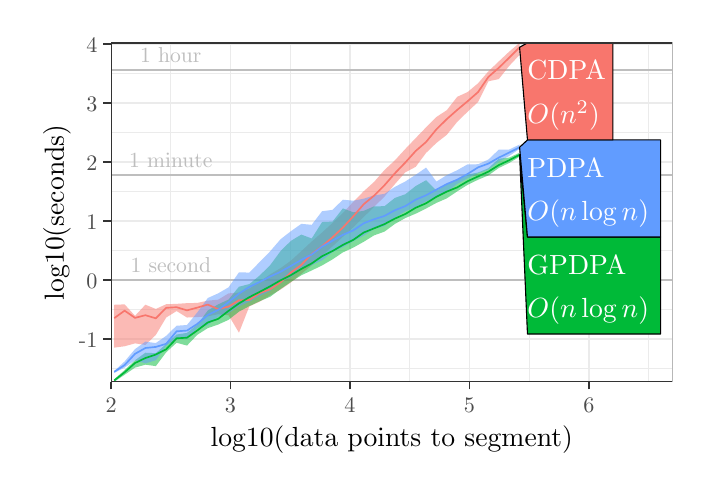
\begin{tikzpicture}[x=1pt,y=1pt]
\definecolor{fillColor}{RGB}{255,255,255}
\path[use as bounding box,fill=fillColor,fill opacity=0.00] (0,0) rectangle (238.49,158.99);
\begin{scope}
\path[clip] (  0.00,  0.00) rectangle (238.49,158.99);
\definecolor{drawColor}{RGB}{255,255,255}
\definecolor{fillColor}{RGB}{255,255,255}

\path[draw=drawColor,line width= 0.6pt,line join=round,line cap=round,fill=fillColor] (  0.00, -0.00) rectangle (238.49,158.99);
\end{scope}
\begin{scope}
\path[clip] ( 30.13, 31.03) rectangle (232.99,153.49);
\definecolor{fillColor}{RGB}{255,255,255}

\path[fill=fillColor] ( 30.13, 31.03) rectangle (232.99,153.49);
\definecolor{drawColor}{gray}{0.92}

\path[draw=drawColor,line width= 0.3pt,line join=round] ( 30.13, 35.75) --
	(232.99, 35.75);

\path[draw=drawColor,line width= 0.3pt,line join=round] ( 30.13, 57.08) --
	(232.99, 57.08);

\path[draw=drawColor,line width= 0.3pt,line join=round] ( 30.13, 78.41) --
	(232.99, 78.41);

\path[draw=drawColor,line width= 0.3pt,line join=round] ( 30.13, 99.74) --
	(232.99, 99.74);

\path[draw=drawColor,line width= 0.3pt,line join=round] ( 30.13,121.08) --
	(232.99,121.08);

\path[draw=drawColor,line width= 0.3pt,line join=round] ( 30.13,142.41) --
	(232.99,142.41);

\path[draw=drawColor,line width= 0.3pt,line join=round] ( 51.71, 31.03) --
	( 51.71,153.49);

\path[draw=drawColor,line width= 0.3pt,line join=round] ( 94.87, 31.03) --
	( 94.87,153.49);

\path[draw=drawColor,line width= 0.3pt,line join=round] (138.03, 31.03) --
	(138.03,153.49);

\path[draw=drawColor,line width= 0.3pt,line join=round] (181.20, 31.03) --
	(181.20,153.49);

\path[draw=drawColor,line width= 0.3pt,line join=round] (224.36, 31.03) --
	(224.36,153.49);

\path[draw=drawColor,line width= 0.6pt,line join=round] ( 30.13, 46.42) --
	(232.99, 46.42);

\path[draw=drawColor,line width= 0.6pt,line join=round] ( 30.13, 67.75) --
	(232.99, 67.75);

\path[draw=drawColor,line width= 0.6pt,line join=round] ( 30.13, 89.08) --
	(232.99, 89.08);

\path[draw=drawColor,line width= 0.6pt,line join=round] ( 30.13,110.41) --
	(232.99,110.41);

\path[draw=drawColor,line width= 0.6pt,line join=round] ( 30.13,131.74) --
	(232.99,131.74);

\path[draw=drawColor,line width= 0.6pt,line join=round] ( 30.13,153.07) --
	(232.99,153.07);

\path[draw=drawColor,line width= 0.6pt,line join=round] ( 30.13, 31.03) --
	( 30.13,153.49);

\path[draw=drawColor,line width= 0.6pt,line join=round] ( 73.29, 31.03) --
	( 73.29,153.49);

\path[draw=drawColor,line width= 0.6pt,line join=round] (116.45, 31.03) --
	(116.45,153.49);

\path[draw=drawColor,line width= 0.6pt,line join=round] (159.62, 31.03) --
	(159.62,153.49);

\path[draw=drawColor,line width= 0.6pt,line join=round] (202.78, 31.03) --
	(202.78,153.49);
\definecolor{drawColor}{RGB}{190,190,190}

\path[draw=drawColor,line width= 0.6pt,line join=round] ( 30.13, 67.75) -- (232.99, 67.75);

\path[draw=drawColor,line width= 0.6pt,line join=round] ( 30.13,105.68) -- (232.99,105.68);

\path[draw=drawColor,line width= 0.6pt,line join=round] ( 30.13,143.61) -- (232.99,143.61);
\definecolor{fillColor}{RGB}{248,118,109}

\path[fill=fillColor,fill opacity=0.50] ( 31.28, 58.86) --
	( 35.03, 59.00) --
	( 38.79, 54.87) --
	( 42.54, 58.88) --
	( 46.30, 57.34) --
	( 50.05, 59.05) --
	( 53.81, 59.19) --
	( 57.57, 59.44) --
	( 61.32, 59.53) --
	( 65.08, 60.35) --
	( 68.83, 60.69) --
	( 72.59, 62.98) --
	( 76.35, 63.26) --
	( 80.10, 64.72) --
	( 83.86, 67.21) --
	( 87.61, 69.85) --
	( 91.37, 72.10) --
	( 95.12, 74.80) --
	( 98.88, 78.24) --
	(102.64, 81.73) --
	(106.39, 84.99) --
	(110.15, 88.42) --
	(113.90, 92.02) --
	(117.66, 96.06) --
	(121.42, 99.87) --
	(125.17,103.24) --
	(128.93,107.55) --
	(132.68,111.03) --
	(136.44,115.14) --
	(140.20,119.07) --
	(143.95,122.96) --
	(147.71,126.72) --
	(151.46,129.18) --
	(155.22,134.00) --
	(158.97,135.72) --
	(162.73,138.88) --
	(166.49,143.21) --
	(170.24,146.80) --
	(174.00,150.33) --
	(177.75,153.49) --
	(177.75,149.16) --
	(174.00,145.18) --
	(170.24,140.42) --
	(166.49,139.61) --
	(162.73,132.12) --
	(158.97,128.62) --
	(155.22,124.98) --
	(151.46,120.29) --
	(147.71,117.36) --
	(143.95,113.73) --
	(140.20,108.69) --
	(136.44,106.71) --
	(132.68,102.45) --
	(128.93, 97.95) --
	(125.17, 94.25) --
	(121.42, 90.58) --
	(117.66, 86.87) --
	(113.90, 83.40) --
	(110.15, 79.97) --
	(106.39, 76.65) --
	(102.64, 73.14) --
	( 98.88, 70.03) --
	( 95.12, 66.90) --
	( 91.37, 64.34) --
	( 87.61, 62.21) --
	( 83.86, 59.99) --
	( 80.10, 58.28) --
	( 76.35, 48.78) --
	( 72.59, 55.09) --
	( 68.83, 55.45) --
	( 65.08, 54.68) --
	( 61.32, 54.41) --
	( 57.57, 54.25) --
	( 53.81, 56.59) --
	( 50.05, 54.25) --
	( 46.30, 47.95) --
	( 42.54, 44.35) --
	( 38.79, 44.91) --
	( 35.03, 43.87) --
	( 31.28, 43.37) --
	cycle;
\definecolor{fillColor}{RGB}{0,186,56}

\path[fill=fillColor,fill opacity=0.50] ( 31.28, 31.96) --
	( 35.03, 35.26) --
	( 38.79, 38.81) --
	( 42.54, 41.53) --
	( 46.30, 41.37) --
	( 50.05, 44.69) --
	( 53.81, 48.11) --
	( 57.57, 48.70) --
	( 61.32, 51.71) --
	( 65.08, 56.81) --
	( 68.83, 59.00) --
	( 72.59, 60.75) --
	( 76.35, 65.39) --
	( 80.10, 66.33) --
	( 83.86, 69.46) --
	( 87.61, 73.14) --
	( 91.37, 78.24) --
	( 95.12, 81.95) --
	( 98.88, 84.23) --
	(102.64, 82.82) --
	(106.39, 88.75) --
	(110.15, 88.91) --
	(113.90, 93.68) --
	(117.66, 92.28) --
	(121.42, 92.80) --
	(125.17, 94.44) --
	(128.93, 94.47) --
	(132.68, 97.46) --
	(136.44, 98.79) --
	(140.20,101.75) --
	(143.95,103.86) --
	(147.71,100.18) --
	(151.46,102.29) --
	(155.22,104.21) --
	(158.97,105.90) --
	(162.73,106.64) --
	(166.49,108.19) --
	(170.24,111.64) --
	(174.00,112.05) --
	(177.75,113.79) --
	(177.75,112.37) --
	(174.00,110.10) --
	(170.24,108.30) --
	(166.49,105.62) --
	(162.73,104.03) --
	(158.97,102.20) --
	(155.22, 99.85) --
	(151.46, 97.31) --
	(147.71, 95.68) --
	(143.95, 93.64) --
	(140.20, 91.78) --
	(136.44, 90.18) --
	(132.68, 88.06) --
	(128.93, 85.29) --
	(125.17, 83.94) --
	(121.42, 81.62) --
	(117.66, 79.52) --
	(113.90, 77.79) --
	(110.15, 75.26) --
	(106.39, 73.08) --
	(102.64, 71.26) --
	( 98.88, 69.52) --
	( 95.12, 67.11) --
	( 91.37, 64.54) --
	( 87.61, 61.74) --
	( 83.86, 60.16) --
	( 80.10, 58.36) --
	( 76.35, 56.38) --
	( 72.59, 53.42) --
	( 68.83, 51.71) --
	( 65.08, 50.42) --
	( 61.32, 48.03) --
	( 57.57, 44.12) --
	( 53.81, 45.13) --
	( 50.05, 41.68) --
	( 46.30, 36.69) --
	( 42.54, 37.21) --
	( 38.79, 36.15) --
	( 35.03, 33.57) --
	( 31.28, 31.03) --
	cycle;
\definecolor{fillColor}{RGB}{97,156,255}

\path[fill=fillColor,fill opacity=0.50] ( 31.28, 34.95) --
	( 35.03, 38.38) --
	( 38.79, 42.84) --
	( 42.54, 45.54) --
	( 46.30, 45.02) --
	( 50.05, 47.63) --
	( 53.81, 51.28) --
	( 57.57, 51.55) --
	( 61.32, 56.12) --
	( 65.08, 61.29) --
	( 68.83, 62.98) --
	( 72.59, 65.16) --
	( 76.35, 70.58) --
	( 80.10, 70.49) --
	( 83.86, 74.34) --
	( 87.61, 78.16) --
	( 91.37, 82.53) --
	( 95.12, 85.44) --
	( 98.88, 88.10) --
	(102.64, 87.75) --
	(106.39, 92.68) --
	(110.15, 93.15) --
	(113.90, 96.83) --
	(117.66, 96.46) --
	(121.42, 97.19) --
	(125.17, 98.37) --
	(128.93, 98.93) --
	(132.68,101.45) --
	(136.44,103.40) --
	(140.20,105.83) --
	(143.95,108.42) --
	(147.71,103.39) --
	(151.46,105.71) --
	(155.22,107.49) --
	(158.97,109.61) --
	(162.73,109.64) --
	(166.49,111.34) --
	(170.24,114.93) --
	(174.00,114.96) --
	(177.75,116.76) --
	(177.75,115.20) --
	(174.00,112.60) --
	(170.24,110.65) --
	(166.49,107.72) --
	(162.73,106.45) --
	(158.97,104.56) --
	(155.22,102.56) --
	(151.46, 99.62) --
	(147.71, 97.74) --
	(143.95, 96.16) --
	(140.20, 94.13) --
	(136.44, 92.65) --
	(132.68, 90.37) --
	(128.93, 87.32) --
	(125.17, 86.24) --
	(121.42, 83.85) --
	(117.66, 81.84) --
	(113.90, 79.70) --
	(110.15, 77.88) --
	(106.39, 74.91) --
	(102.64, 73.20) --
	( 98.88, 71.72) --
	( 95.12, 68.86) --
	( 91.37, 67.00) --
	( 87.61, 63.83) --
	( 83.86, 62.01) --
	( 80.10, 59.93) --
	( 76.35, 58.33) --
	( 72.59, 55.82) --
	( 68.83, 54.57) --
	( 65.08, 51.55) --
	( 61.32, 50.42) --
	( 57.57, 46.60) --
	( 53.81, 46.69) --
	( 50.05, 44.12) --
	( 46.30, 38.81) --
	( 42.54, 37.69) --
	( 38.79, 38.81) --
	( 35.03, 36.15) --
	( 31.28, 34.29) --
	cycle;
\definecolor{drawColor}{RGB}{248,118,109}

\path[draw=drawColor,line width= 0.6pt,line join=round] ( 31.28, 54.03) --
	( 35.03, 56.73) --
	( 38.79, 54.13) --
	( 42.54, 55.09) --
	( 46.30, 53.97) --
	( 50.05, 57.75) --
	( 53.81, 57.98) --
	( 57.57, 56.84) --
	( 61.32, 57.84) --
	( 65.08, 58.93) --
	( 68.83, 57.26) --
	( 72.59, 58.21) --
	( 76.35, 60.49) --
	( 80.10, 60.60) --
	( 83.86, 63.09) --
	( 87.61, 64.46) --
	( 91.37, 66.99) --
	( 95.12, 70.53) --
	( 98.88, 73.27) --
	(102.64, 77.22) --
	(106.39, 80.02) --
	(110.15, 83.23) --
	(113.90, 86.76) --
	(117.66, 90.82) --
	(121.42, 95.19) --
	(125.17, 98.29) --
	(128.93,102.05) --
	(132.68,106.35) --
	(136.44,110.24) --
	(140.20,114.43) --
	(143.95,117.67) --
	(147.71,122.28) --
	(151.46,125.96) --
	(155.22,129.28) --
	(158.97,132.41) --
	(162.73,135.70) --
	(166.49,141.20) --
	(170.24,144.49) --
	(174.00,148.14) --
	(177.75,151.90);
\definecolor{drawColor}{RGB}{0,186,56}

\path[draw=drawColor,line width= 0.6pt,line join=round] ( 31.28, 31.51) --
	( 35.03, 34.46) --
	( 38.79, 37.81) --
	( 42.54, 39.62) --
	( 46.30, 40.88) --
	( 50.05, 42.78) --
	( 53.81, 46.74) --
	( 57.57, 46.96) --
	( 61.32, 49.60) --
	( 65.08, 52.46) --
	( 68.83, 53.76) --
	( 72.59, 56.67) --
	( 76.35, 59.35) --
	( 80.10, 61.61) --
	( 83.86, 63.54) --
	( 87.61, 65.53) --
	( 91.37, 67.70) --
	( 95.12, 69.57) --
	( 98.88, 71.81) --
	(102.64, 73.80) --
	(106.39, 76.41) --
	(110.15, 78.27) --
	(113.90, 80.49) --
	(117.66, 82.30) --
	(121.42, 84.96) --
	(125.17, 86.47) --
	(128.93, 88.00) --
	(132.68, 89.99) --
	(136.44, 91.65) --
	(140.20, 93.91) --
	(143.95, 95.53) --
	(147.71, 97.89) --
	(151.46, 99.76) --
	(155.22,101.28) --
	(158.97,103.50) --
	(162.73,105.23) --
	(166.49,106.97) --
	(170.24,109.33) --
	(174.00,111.09) --
	(177.75,113.07);
\definecolor{drawColor}{RGB}{97,156,255}

\path[draw=drawColor,line width= 0.6pt,line join=round] ( 31.28, 34.62) --
	( 35.03, 37.08) --
	( 38.79, 41.13) --
	( 42.54, 43.24) --
	( 46.30, 43.63) --
	( 50.05, 44.75) --
	( 53.81, 49.27) --
	( 57.57, 49.53) --
	( 61.32, 51.96) --
	( 65.08, 55.16) --
	( 68.83, 57.00) --
	( 72.59, 59.81) --
	( 76.35, 62.89) --
	( 80.10, 65.32) --
	( 83.86, 67.10) --
	( 87.61, 69.06) --
	( 91.37, 70.77) --
	( 95.12, 72.90) --
	( 98.88, 75.08) --
	(102.64, 77.03) --
	(106.39, 79.87) --
	(110.15, 82.00) --
	(113.90, 84.13) --
	(117.66, 85.74) --
	(121.42, 88.31) --
	(125.17, 89.75) --
	(128.93, 90.96) --
	(132.68, 93.01) --
	(136.44, 94.50) --
	(140.20, 96.83) --
	(143.95, 98.42) --
	(147.71,100.48) --
	(151.46,102.49) --
	(155.22,104.07) --
	(158.97,106.13) --
	(162.73,108.50) --
	(166.49,109.87) --
	(170.24,112.03) --
	(174.00,113.86) --
	(177.75,115.78);
\definecolor{drawColor}{RGB}{190,190,190}

\node[text=drawColor,anchor=base,inner sep=0pt, outer sep=0pt, scale=  0.78] at ( 51.71, 70.67) {1 second};

\node[text=drawColor,anchor=base,inner sep=0pt, outer sep=0pt, scale=  0.78] at ( 51.71,108.60) {1 minute};

\node[text=drawColor,anchor=base,inner sep=0pt, outer sep=0pt, scale=  0.78] at ( 51.71,146.53) {1 hour};
\end{scope}
\begin{scope}
\path[clip] ( 30.13, 31.03) rectangle (232.99,153.49);
\definecolor{drawColor}{RGB}{0,0,0}
\definecolor{fillColor}{RGB}{0,186,56}

\path[draw=drawColor,line width= 0.4pt,line join=round,line cap=round,fill=fillColor] (177.75,113.07) --
	(180.60, 83.35) --
	(228.71, 83.35) --
	(228.71, 48.28) --
	(180.60, 48.28) --
	cycle;
\definecolor{fillColor}{RGB}{97,156,255}

\path[draw=drawColor,line width= 0.4pt,line join=round,line cap=round,fill=fillColor] (177.75,115.78) --
	(180.60,118.42) --
	(228.71,118.42) --
	(228.71, 83.35) --
	(180.60, 83.35) --
	cycle;
\definecolor{fillColor}{RGB}{248,118,109}

\path[draw=drawColor,line width= 0.4pt,line join=round,line cap=round,fill=fillColor] (177.75,151.90) --
	(180.60,153.49) --
	(211.44,153.49) --
	(211.44,118.42) --
	(180.60,118.42) --
	cycle;
\definecolor{drawColor}{RGB}{255,255,255}

\node[text=drawColor,anchor=base west,inner sep=0pt, outer sep=0pt, scale=  1.00] at (180.60, 69.96) {GPDPA};

\node[text=drawColor,anchor=base west,inner sep=0pt, outer sep=0pt, scale=  1.00] at (180.60, 54.12) {$O(n \log n)$};

\node[text=drawColor,anchor=base west,inner sep=0pt, outer sep=0pt, scale=  1.00] at (180.60,105.03) {PDPA};

\node[text=drawColor,anchor=base west,inner sep=0pt, outer sep=0pt, scale=  1.00] at (180.60, 89.19) {$O(n \log n)$};

\node[text=drawColor,anchor=base west,inner sep=0pt, outer sep=0pt, scale=  1.00] at (180.60,140.11) {CDPA};

\node[text=drawColor,anchor=base west,inner sep=0pt, outer sep=0pt, scale=  1.00] at (180.60,124.27) {$O(n^2)$};
\definecolor{drawColor}{gray}{0.20}

\path[draw=drawColor,line width= 0.6pt,line join=round,line cap=round] ( 30.13, 31.03) rectangle (232.99,153.49);
\end{scope}
\begin{scope}
\path[clip] (  0.00,  0.00) rectangle (238.49,158.99);
\definecolor{drawColor}{gray}{0.30}

\node[text=drawColor,anchor=base east,inner sep=0pt, outer sep=0pt, scale=  0.80] at ( 25.18, 43.40) {-1};

\node[text=drawColor,anchor=base east,inner sep=0pt, outer sep=0pt, scale=  0.80] at ( 25.18, 64.73) {0};

\node[text=drawColor,anchor=base east,inner sep=0pt, outer sep=0pt, scale=  0.80] at ( 25.18, 86.06) {1};

\node[text=drawColor,anchor=base east,inner sep=0pt, outer sep=0pt, scale=  0.80] at ( 25.18,107.39) {2};

\node[text=drawColor,anchor=base east,inner sep=0pt, outer sep=0pt, scale=  0.80] at ( 25.18,128.72) {3};

\node[text=drawColor,anchor=base east,inner sep=0pt, outer sep=0pt, scale=  0.80] at ( 25.18,150.06) {4};
\end{scope}
\begin{scope}
\path[clip] (  0.00,  0.00) rectangle (238.49,158.99);
\definecolor{drawColor}{gray}{0.20}

\path[draw=drawColor,line width= 0.6pt,line join=round] ( 27.38, 46.42) --
	( 30.13, 46.42);

\path[draw=drawColor,line width= 0.6pt,line join=round] ( 27.38, 67.75) --
	( 30.13, 67.75);

\path[draw=drawColor,line width= 0.6pt,line join=round] ( 27.38, 89.08) --
	( 30.13, 89.08);

\path[draw=drawColor,line width= 0.6pt,line join=round] ( 27.38,110.41) --
	( 30.13,110.41);

\path[draw=drawColor,line width= 0.6pt,line join=round] ( 27.38,131.74) --
	( 30.13,131.74);

\path[draw=drawColor,line width= 0.6pt,line join=round] ( 27.38,153.07) --
	( 30.13,153.07);
\end{scope}
\begin{scope}
\path[clip] (  0.00,  0.00) rectangle (238.49,158.99);
\definecolor{drawColor}{gray}{0.20}

\path[draw=drawColor,line width= 0.6pt,line join=round] ( 30.13, 28.28) --
	( 30.13, 31.03);

\path[draw=drawColor,line width= 0.6pt,line join=round] ( 73.29, 28.28) --
	( 73.29, 31.03);

\path[draw=drawColor,line width= 0.6pt,line join=round] (116.45, 28.28) --
	(116.45, 31.03);

\path[draw=drawColor,line width= 0.6pt,line join=round] (159.62, 28.28) --
	(159.62, 31.03);

\path[draw=drawColor,line width= 0.6pt,line join=round] (202.78, 28.28) --
	(202.78, 31.03);
\end{scope}
\begin{scope}
\path[clip] (  0.00,  0.00) rectangle (238.49,158.99);
\definecolor{drawColor}{gray}{0.30}

\node[text=drawColor,anchor=base,inner sep=0pt, outer sep=0pt, scale=  0.80] at ( 30.13, 20.05) {2};

\node[text=drawColor,anchor=base,inner sep=0pt, outer sep=0pt, scale=  0.80] at ( 73.29, 20.05) {3};

\node[text=drawColor,anchor=base,inner sep=0pt, outer sep=0pt, scale=  0.80] at (116.45, 20.05) {4};

\node[text=drawColor,anchor=base,inner sep=0pt, outer sep=0pt, scale=  0.80] at (159.62, 20.05) {5};

\node[text=drawColor,anchor=base,inner sep=0pt, outer sep=0pt, scale=  0.80] at (202.78, 20.05) {6};
\end{scope}
\begin{scope}
\path[clip] (  0.00,  0.00) rectangle (238.49,158.99);
\definecolor{drawColor}{RGB}{0,0,0}

\node[text=drawColor,anchor=base,inner sep=0pt, outer sep=0pt, scale=  1.00] at (131.56,  7.63) {log10(data points to segment)};
\end{scope}
\begin{scope}
\path[clip] (  0.00,  0.00) rectangle (238.49,158.99);
\definecolor{drawColor}{RGB}{0,0,0}

\node[text=drawColor,rotate= 90.00,anchor=base,inner sep=0pt, outer sep=0pt, scale=  1.00] at ( 13.04, 92.26) {log10(seconds)};
\end{scope}
\end{tikzpicture}
